	\begin{center}
		\begin{tikzpicture}
			\draw[thick, fill=gray!30] (-1.7, -3.5) rectangle +(2, 1);
			\draw[thick, fill = white] (-1.4, -3.1) rectangle +(0.2, 0.3);
			\draw[thick, fill = white] (-0.8, -3.1) rectangle +(0.2, 0.3);			
			\draw[thick] (-93:0.7) -- (-93:2.5);
			\draw[thick] (-87:0.7) -- (-87:2.5);
			\draw[fill=red, opacity = 0.6] (-93:0.7) -- (-93:1) arc(-93:-87:1) -- (-87:0.7) arc(-87:-93:0.7);
			\draw[fill=red, opacity = 0.6] (-93:1.3) -- (-93:1.6) arc(-93:-87:1.6) -- (-87:1.3) arc(-87:-93:1.3);
			\draw[fill=red, opacity = 0.6] (-93:1.9) -- (-93:2.2) arc(-93:-87:2.2) -- (-87:1.9) arc(-87:-93:1.9);
			\draw[fill=blue, opacity = 0.7] (0.2, -0.6) -- (1.7, -0.6) -- (1.7, 0.4) -- cycle;
			\draw[fill=green, opacity = 0.4] (6.2, -0.6) -- (7.7, -0.6) -- (7.7, 0.4) -- cycle;
			\draw[<->, dashed] (0.2, -0.7) -- (1.7, -0.7)node[midway, below]{$100\text{ м}$};
			\draw[<->, dashed] (1.7, -0.9) -- (6.2, -0.9)node[midway, below]{$1\text{ км}$};
			\draw[<->, dashed] (6.2, -0.7) -- (7.7, -0.7)node[midway, below]{$100\text{ м}$};
			\draw[->] (1.75, -0.1) -- (2.7, -0.1)node[midway, above]{$15\text{ м/с}$};
			\draw[->] (7.75, -0.1) -- (8.7, -0.1)node[midway, above]{$5\text{ м/с}$};
		\end{tikzpicture}
	\end{center}
Обозначим длину основания облака $l$, а начальное расстояние между облаками $L$. Скорости облаков $v_1$ и $v_2$.
Скорость их сближения $v_{\text{сбл}} = v_2 - v_1$.

Разобьем движение на несколько частей. Рассмотрим первую из них, во время которой снег выпадать не будет. На ней левое облако догоняет правое до того момента, когда между ними произойдет контакт. На это требуется время, равное
\begin{equation}
	t_1 = \frac{L}{v_{\text{сбл}}} = \frac{1\text{ км}}{10\text{м/с}} = 100\text{с}.
\end{equation} 

После этого между контактирующими частями облаков будет происходить взаимодействие, которое стоит рассмотреть более подробно. Понятно, что снег будет образовываться на границе, разделяющей различные вещества, и следует понять, как эта граница будет располагаться в пространстве.

Рассмотрим для начала более простой случай, когда облака имеют форму прямоугольников, движущихся навстречу друг другу с одинаковыми скоростями.
\begin{center}
	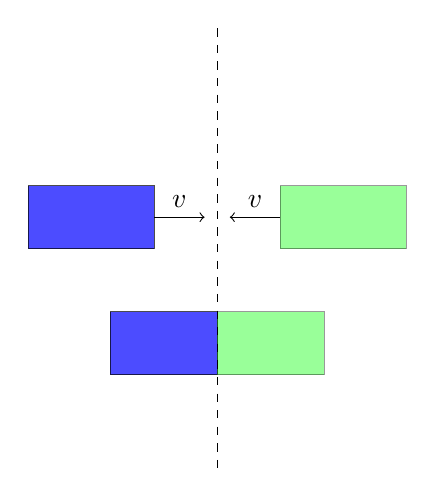
\begin{tikzpicture}[scale=0.8]
		\draw[fill = blue, opacity = 0.7] (-3, 0) rectangle +(2, 1);
		\draw[fill = green, opacity = 0.4] (3, 0) rectangle +(-2, 1);
		\draw[->] (-1, 0.5) -- (-0.2, 0.5)node[midway, above]{$v$};
		\draw[->] (1, 0.5) -- (0.2, 0.5)node[midway, above]{$v$};
		\draw[fill = blue, opacity = 0.7] (-1.7, -2) rectangle +(1.7, 1);
		\draw[fill = green, opacity = 0.4] (1.7, -2) rectangle +(-1.7, 1);
		\draw[dashed] (0, 3.5) -- (0, -3.5);
	\end{tikzpicture}
\end{center}

Понятно, что в таком случае из соображений симметрии можно сказать, что граница контакта будет оставаться на одном месте и быть точно посередине между внешними вертикальными границами облаков. 

Если перейти в систему отсчета, в которой левое облако покоится, то после контакта его левая граница будет неподвижна, а линия контакта будет двигаться влево со скоростью $v$, то есть с вдвое меньшей, чем правое облако в этой системе отчета.
\begin{figure}[h!]
	\centering
	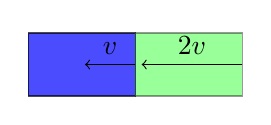
\begin{tikzpicture}[scale=0.8]
		\draw[fill = blue, opacity = 0.7] (-1.7, 0) rectangle +(1.7, 1);
		\draw[fill = green, opacity = 0.4] (1.7, 0) rectangle +(-1.7, 1);
		\draw[->] (0, 0.5) -- (-0.8, 0.5)node[midway, above]{$v$};
		\draw[->] (1.7, 0.5) -- (0.1, 0.5)node[midway, above]{$2v$};
	\end{tikzpicture}
	\caption*{Два прямоугольных облака в системе отсчета, где левое облако покоится.}
\end{figure}

Теперь вернемся к нашему случаю. Представим треугольники как лесенки с очень мелкими ступеньками. Тогда можно понять, как взаимодействуют отдельные прямоугольники, образующие ступеньки и найти, в итоге, как будет располагаться граница раздела. Удобно рассматривать процесс в системе отсчета левого облака.
\begin{center}
	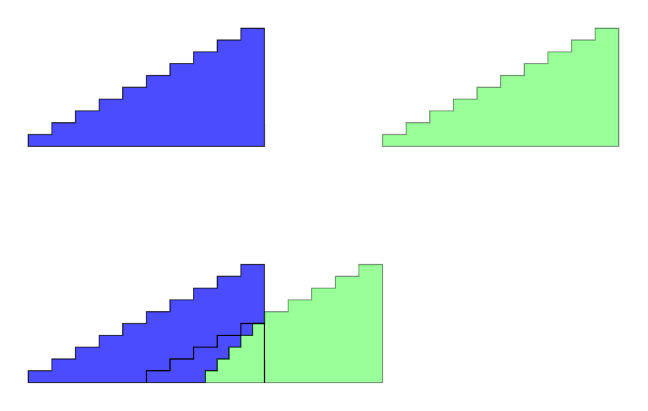
\begin{tikzpicture}[scale = 1.5]
		\draw[fill = blue, opacity = 0.7] (0, 0) -- (-2, 0) \foreach \i in {1,2,...,10}{ -- ++(0, 0.1) -- ++(0.2, 0)} -- cycle; 
		\draw[fill = green, opacity = 0.4] (3, 0) -- (1, 0) \foreach \i in {1,2,...,10}{ -- ++(0, 0.1) -- ++(0.2, 0)} -- cycle;
		\draw[fill = blue, opacity = 0.7] (-0.5, -2) -- (-2, -2) \foreach \i in {1,2,...,10}{ -- ++(0, 0.1) -- ++(0.2, 0)} -- (0, -1.5) \foreach \i in {1,2,...,5}{-- ++(-0.1, 0) -- ++(0, -0.1)} ; 
		\draw[fill = green, opacity = 0.4] (1, -2) -- (-0.5, -2) \foreach \i in {1,2,...,5}{ -- ++(0, 0.1) -- ++(0.1, 0)} \foreach \i in {1,2,...,5}{ -- ++(0, 0.1) -- ++(0.2, 0)} -- cycle;
		\draw (-1, -2) \foreach \i in {1,2,...,5}{ -- ++(0, 0.1) -- ++(0.2, 0)} -- (0, -2);
	\end{tikzpicture}
\end{center}

Видно, что каждая грань ступеньки, соприкасаясь со вторым облаком, начинает двигаться вдвое медленнее. Тогда, если вернуться к непрерывному рассмотрению, границей раздела будет участок прямой, имеющей вдвое больший коэффициент наклона, чем наклонная сторона треугольника.
\begin{center}
	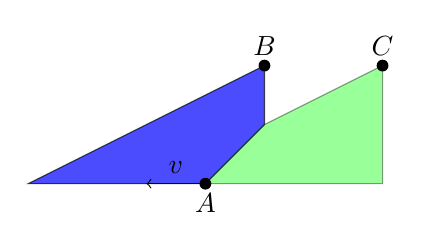
\begin{tikzpicture}[scale = 1.5]
		\draw[fill = blue, opacity = 0.7] (0, 1) -- (0, 0.5) -- (-0.5, 0) -- (-2, 0) -- cycle;
		\draw[fill = green, opacity = 0.4] (-0.5, 0) -- (0, 0.5) -- (1, 1) -- (1, 0) -- cycle;
		\fill (-0.5, 0)node[below]{$A$} circle(0.05);
		\fill (0, 1)node[above]{$B$} circle(0.05);
		\fill (1, 1)node[above]{$C$} circle(0.05);
		\draw[->] (-0.5, 0) -- (-1, 0)node[midway, above]{$v$};
	\end{tikzpicture}
\end{center}
Точка $A$ на нижней стороне облака, через которую проходит граница раздела будет двигаться со скоростью $v=\frac{v_{\text{сбл}}}{2}$. 

Можно понять, что количество выпадающего снега в единицу времени равно числу провзаимодействовавших частиц, а оно пропорционально высоте границы раздела. Тогда нужно найти момент времени, в который высота границы раздела максимальна. Ясно, что это тот момент, когда граница проходит через вершину $B$ треугольника. В этот момент вершина правого облака (точка $C$) совпадает с точкой $B$. Точка $A$ в этот момент дойдет до середины основания, а это займет время
\begin{equation}
	t_2 = \frac{\frac{l}{2}}{\frac{v_{\text{сбл}}}{2}} = \frac{l}{v_{\text{сбл}}} = \frac{100\text{ м}}{10\text{ м/с}} =10\text{ с}.
\end{equation}

\begin{center}
	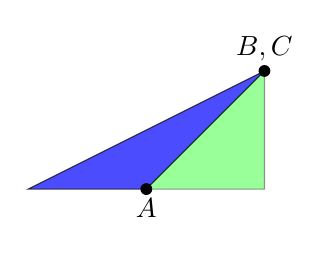
\begin{tikzpicture}[scale = 1.5]
		\draw[fill = blue, opacity = 0.7] (0, 1) -- (-1, 0) -- (-2, 0) -- cycle;
		\draw[fill = green, opacity = 0.4] (0, 1) -- (0, 0) -- (-1, 0) -- cycle;
		\fill (-1, 0)node[below]{$A$} circle(0.05);
		\fill (0, 1)node[above]{$B,C$} circle(0.05);
	\end{tikzpicture}	
\end{center}

Тогда в сумме с начала движения до искомого момента пройдет
\begin{equation}
	t = t_1 + t_2 = 110\text{ с}.
\end{equation} 

После этого момента снег идти не перестанет, так как не провзаимодействовавшие части облаков еще остались. Снег будет идти, начиная с момента касания, и до того момента, как точка $A$ дойдет до левой границы основания. На это понадобится время
\begin{equation}
	t'_2 = \frac{l}{v_{\text{сбл}}} = \frac{100\text{ м}}{5\text{ м/с}} =20\text{ с}
\end{equation}
\olympanswer{ Максимум выпадения в момент $110$ с, продолжительность снегопада --- $20$ c.}

\ifgrade
\begin{grade-env}
	\grade{1}{Нахождение $v_{\text{сбл}}$,}
	\grade{1}{Нахождение $t_1$,}
	\grade{3}{Ставится за понимание того, что происходит с облаком после момента максимума,}
	\grade{1}{Ответ для продолжительности,}
	\grade{2}{Ответ для момента времени (балл ставится, если нахождение этого момента обосновано и непротиворечиво).}
\end{grade-env}
\fi